% Two-node right Radau basis: ellbar_1=1.5(1-tau), Omega_1=1.5tau-.75tau^2.
% The shaded area is the value of the integral at the marked coordinate.
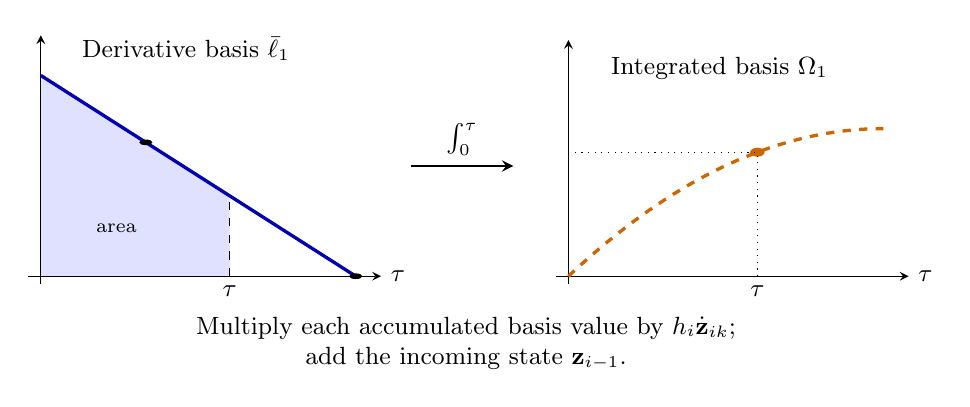
\begin{tikzpicture}[>=stealth,x=1cm,y=1cm,font=\small]
\begin{scope}[xscale=4,yscale=1.7]
\fill[blue!12] (0,0)--plot[domain=0:.6,samples=30](\x,{1.5*(1-\x)})--(.6,0)--cycle;
\draw[->,black](-.04,0)--(1.08,0)node[right]{$\tau$};
\draw[->,black](0,-.06)--(0,1.8);
\draw[blue!70!black,very thick,domain=0:1]plot(\x,{1.5*(1-\x)});
\draw[dashed](.6,0)--(.6,.6);
\fill(.333333,1)circle(.6pt);\fill(1,0)circle(.6pt);
\node[anchor=west]at(.1,1.7){Derivative basis $\bar\ell_1$};
\node[below]at(.6,0){$\tau$};
\node[font=\scriptsize]at(.24,.36){area};
\end{scope}
\draw[->,thick](4.7,1.4)--(6,1.4)node[midway,above]{$\int_0^\tau$};
\begin{scope}[shift={(6.7,0)},xscale=4,yscale=2.5]
\draw[->,black](-.04,0)--(1.08,0)node[right]{$\tau$};
\draw[->,black](0,-.04)--(0,1.2);
\draw[orange!80!black,very thick,dashed,domain=0:1,samples=40]plot(\x,{1.5*\x-.75*\x*\x});
\fill[orange!80!black](.6,.63)circle(.65pt);
\draw[dotted](.6,0)--(.6,.63)--(0,.63);
\node[above]at(.48,.95){Integrated basis $\Omega_1$};
\node[below]at(.6,0){$\tau$};
\end{scope}
\node[align=center]at(5.4,-.85){Multiply each accumulated basis value by $h_i\dot{\mathbf z}_{ik}$;\\add the incoming state $\mathbf z_{i-1}$.};
\end{tikzpicture}
